\documentclass[11pt, oneside]{article}   	% use "amsart" instead of "article" for AMSLaTeX format
\usepackage{geometry}                		% See geometry.pdf to learn the layout options. There are lots.
\geometry{letterpaper}                   		% ... or a4paper or a5paper or ... 
%\geometry{landscape}                		% Activate for rotated page geometry
%\usepackage[parfill]{parskip}    		% Activate to begin paragraphs with an empty line rather than an indent
\usepackage{graphicx}				% Use pdf, png, jpg, or eps§ with pdflatex; use eps in DVI mode
								% TeX will automatically convert eps --> pdf in pdflatex		
\usepackage{amssymb}
\usepackage{minted}
%SetFonts

%SetFonts


\title{Brief Article}
\author{The Author}
%\date{}							% Activate to display a given date or no date

\begin{document}
\begin{flushright}
Donovan Guelde\\
CSCI 5352\\
PS 5\\
\end{flushright}
1. a.  To investigate the "guilt by association" (GbA) heuristic, the experiment as described in Problem Set 5, question 1.a. was performed on the "Norwegian Board of Directors (2002-2011, projection)", network net1m\_2011-08-01, and the "Malaria var DBLa HVR networks", network HVR\_5.  To achieve consistent results, 1000 iterations were performed and results averaged for each $f$ value tested, $f$ being the fraction of vertex nodes that were visible.  The range of $f$ values was [0.01,0.99], and $f$ was increased in increments of 0.02, giving 50 data points.  Results for network net1m\_2011-08-01 are as follows:\\
\begin{center} Accuracy as a Function of $f$ for GbA Heuristic on net1m\_2011-08-01 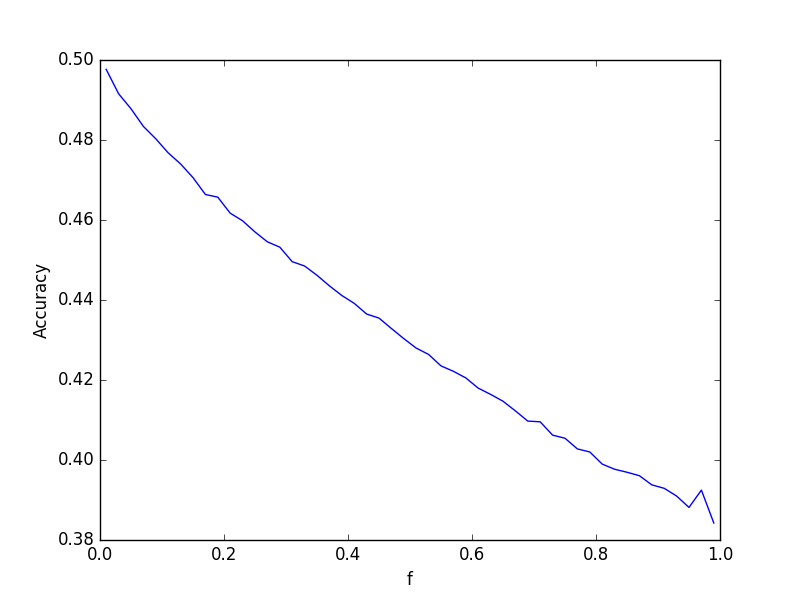
\includegraphics[scale=0.6]{net1m_2011-08-011000Iterations.png}\end{center}
\
\indent At $f$=0.01, accuracy is very nearly 0.5, which is expected.  This network has vertices labeled by gender, and a simple random choice is expected to produce an accuracy of 0.5 in a binary classification.  As $f$ increases, the accuracy of the GbA heuristic decreases, to a minimum of 0.384.  This may seem surprising, considering that board membership is male-dominated in the United States, with only 17.9\% of board seats filled by women(https:\/\/en.wikipedia.org/wiki/Gender\_representation\_on\_corporate\_boards\_of\_directors).  However, it is important to view these results while taking recent history into account, particularly the enactment in Norway of a gender representation law requiring at least 40\% representation of each gender in corporate boards (https://toreopsahl.com/2010/09/30/article-for-the-few-not-the-many-the-effects-of-affirmative-action-on-presence-prominence-and-social-capital-of-women-directors-in-norway/).  Such heavy mixing of genders drastically lowers the accuracy of the GbA heuristic.  Corporate boards dominated by males, as in the US, but neither are they dominated by women, either (as per the Norwegian law).  The results shown by the above graph show that nodes in the net1m\_2011-08-01 network do not exhibit homophily.\\\\
\begin{center} Accuracy as a Function of $f$ for GbA Heuristic on network HVR\_5 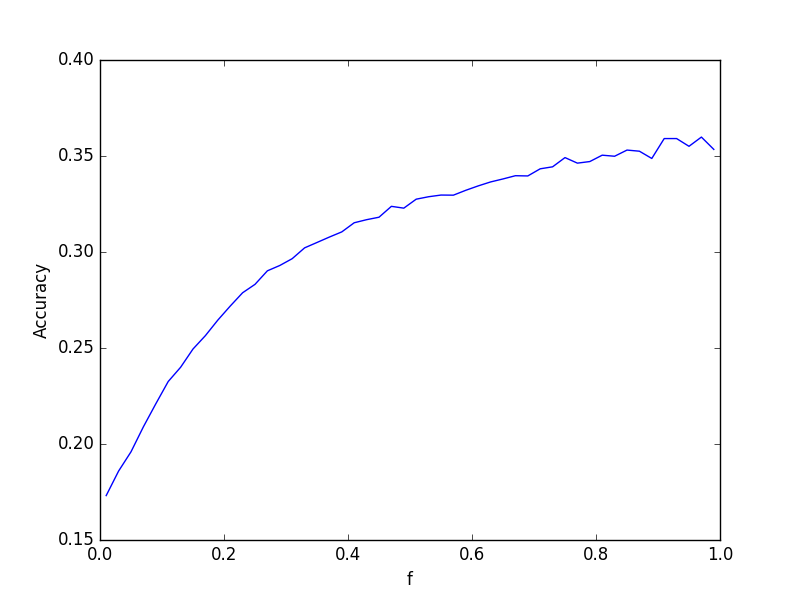
\includegraphics[scale=0.6]{HVR_51000Iterations.png}\end{center}
\indent\indent The results of GbA on network HVR\_5 show similarly expected results at an $f$ value near 0.0.  This network uses six unique node labels, and a random assignment of labels can be expected to be correct $\frac{1}{6}$ (0.166667) of the time.  As $f$ increases, accuracy also increases, up to 0.353.  While this is still a relatively low accuracy, it is more than double that of random assignment.  This indicates that vertices in the HVR\_5 network do show some degree of homophily.  This conclusion appears to be supported by the following visualization of the HVR\_5 network(http://danlarremore.com/var/), linked to by the paper associated with the network file (D. B. Larremore, A. Clauset, and C. O. Buckee, "A network approach to analyzing highly recombinant malaria parasite genes." PLOS Computational Biology 9(10), e1003268 (2013).)\\
\begin{center}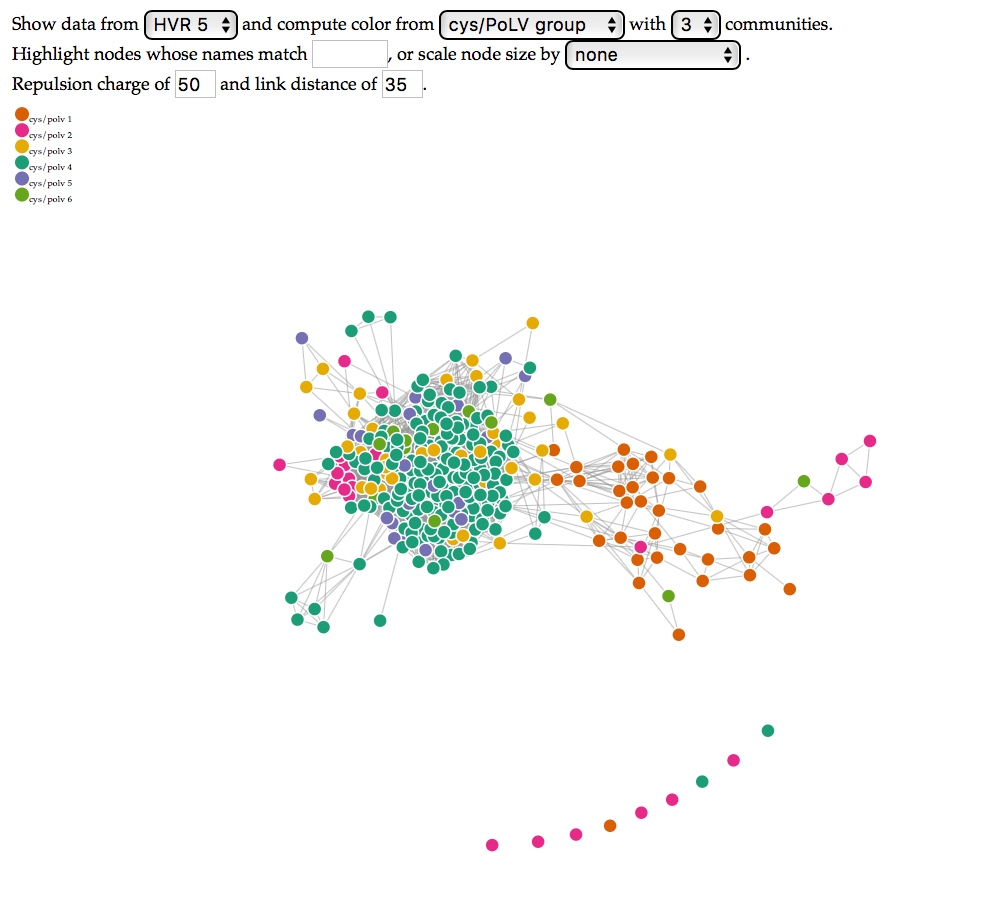
\includegraphics[scale=0.3]{grab}\end{center}
\indent\indent From this visualization, it appears that the homophily in this network may be largely driven by the 'cyc/polv. 4' nodes.  Nodes with this label appear to be the most numerous and have a high degree of homophily.\\


\indent One interesting aspect of the results from both networks is the decrease in smoothness of the plots as $f$ nears 1.0.  This can possibly be explained by the drastically reduced size of the test set.  As $f$ approaches 1.0, the size of the test set approaches 0 (a fact that I had to account for in coding for this question, as a test set of size 0 would cause my code to crash).  With such a small test set size, variance of results increases, even with 1000 repetitions per value of $f$.\\\\\\
1. b.  Utilizing the three scoring functions described in Problem Set 5, question 1.b., accuracy of edge prediction was investigated on the networks net1m\_2011-08-01 and HVR\_5.  Accuracy, as determined by AUC, was measured over 10 iterations per $f$ value, where $f$=[0.01,0.99], increased in increments of 0.02.  The scikit learn roc\_auc\_score() function was used to calculate AUC value.\\\\\\\\
\begin{center}Accuracy (AUC) as a Function of $f$ for Edge Prediction\\via Three Scoring Methods on net1m\_2011-08-01 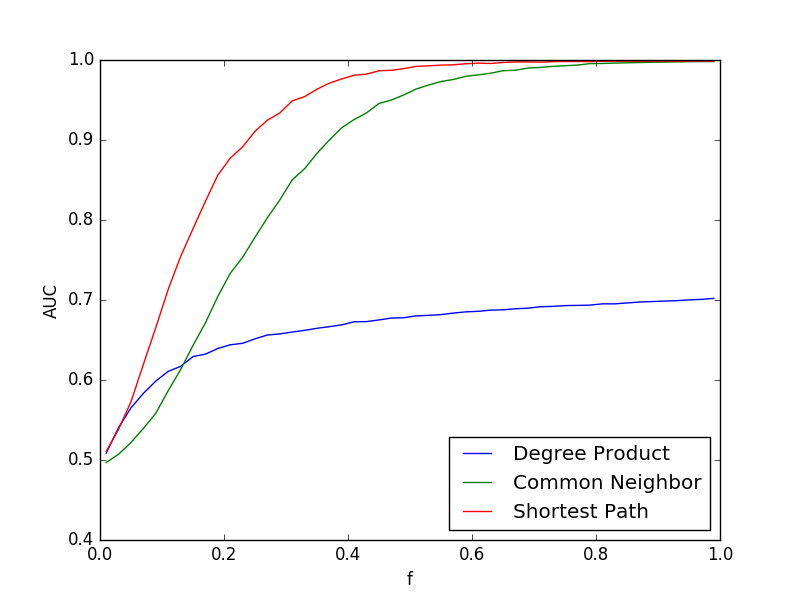
\includegraphics[scale=0.5]{predictEdgesnet1m_2011-08-0110Iterations.png}\end{center}
\indent\indent The accuracy of the common neighbor and shortest path scoring systems, as determined by UAC, increases rapidly for the net1m\_2011-08-01 network.  This network is a projection of a bipartite graph, and as such, vertices(board members) who sit on the same board (vertices that are linked to the same node in the bipartite network) form a clique in the simple network.  Therefore, common neighbor and shortest path scores provide an excellent link predictor.  All vertices on the same board (same bipartite network pairing) have a shortest path distance of 1(2 if the linking edge has been hidden), and share all of the same common neighbors (common neighbor score of 1 by our scoring methodology).  By similar reasoning, degree product should also be a good predictor, since board members in the same clique likely have a common degree.  The predictive power of the degree product score is lessened by the fact that individuals may sit on multiple corporate boards, lessening the correlation of board membership and degree.  Different boards may also have the same number of members, giving possibly unconnected cliques the same degree product scores.\\\\\\\\\\\\\\\\
\begin{center}Accuracy (AUC) as a Function of $f$ for Edge Prediction\\via Three Scoring Methods on HVR\_5 Network 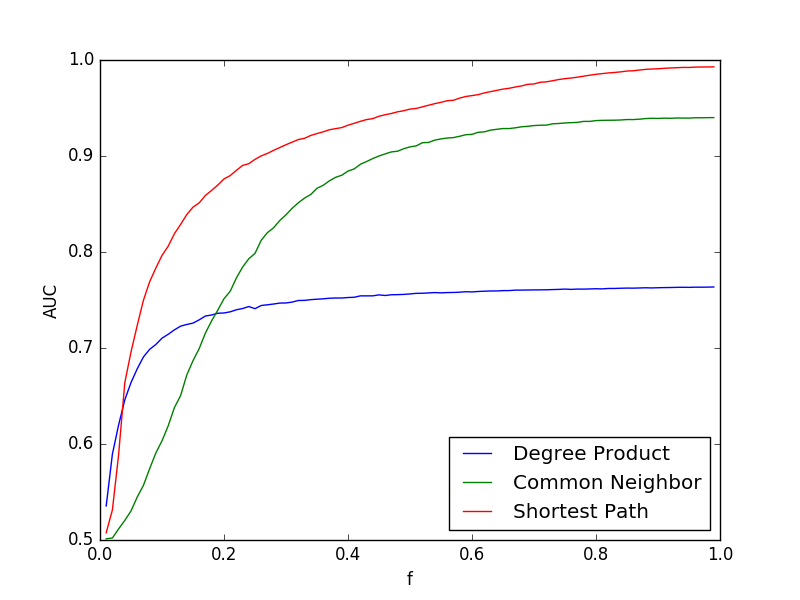
\includegraphics[scale=0.5]{predictEdgesHVR_520Iterations.png}\end{center}
\indent\indent The HVR\_5 network shows similar edge prediction results as the net1m\_2011-08-01 network.  As we saw in question 1.a., the HVR\_5 network shows strong homophily among like vertices.  This homophily is analogous to the cliques formed in net1m\_2011-08-01, making common neighbor and shortest path scores good edge predictors, while degree product is a weaker predictor.  Due to the apparent absence of strong cliques that are present in net1m\_2011-08-01, prediction accuracy of shortest path and common neighbor are not as strong as they are in network net1m\_2011-08-01.\\\\\\
2.  To answer question 2, the Yeast transcription network (2002)  and the US airport networks (2010) (complete US airport network in 2010) were used.  To get accurate results on average cascade size, 2,000 iterations were performed for each node as 'Patient Zero'.\\\\\\\\\\\\\\\\\\\\

\begin{center} US airport Network results:\\
\begin{tabular}{c|c|c|c}
\hline
Node & Airport & Average Cascade Size&Degree\\
\hline
114& Atlanta International & 9.5275& 314\\
\hline
709& Dulles International & 8.968&299\\
\hline
1200&Chicago O'Hare & 8.9295&296\\
\hline
766&John F. Kennedy International & 8.824&291\\
\hline
877&Los Angeles International & 8.754&292\\
\hline
389&Denver International & 8.4115&274\\
\hline
500&Newark Liberty International & 8.3655&273\\
\hline
1068& Minneapolis Saint Paul International & 8.2405&269\\
\hline
711&George Bush Intercontinental (Houston) & 8.209&267\\
\hline
1016& Miami International& 8.0385&261\\
\hline
\end{tabular}
\end{center}
\indent\indent Cascade size for the US airport network reflects the relative importance of airports in the US.  The airport network is made up of a number of large 'hubs' that connect to other hubs, as well as smaller, regional airports.  Therefore, these large hub airports are more likely to be the starting point for the largest cascades.  Due to the low probability of transmission of $\frac{1}{c}=\frac{1}{37.061}$, only the largest airports can be expected to spread to even one or two neighboring nodes.  The probability of a small regional airport infecting even one neighbor is approaching zero.  Only the largest airports, linking to other very large hubs, are able to start a cascade that will reliably spread.  A small airport may be able to occasionally spread a cascade to a large hub, but not reliably, over multiple iterations of the simulation.  The degree of the airport nodes correlates very well with cascade size and ranking, with the lone exception being node 766, JFK International, that has degree one less than the next node.  This can easily be explained by JFK having fewer connections to smaller airports, which do not help to spread the cascade.\\\\\\\\\\\\\\\\\\\\\\\\
\begin{center} Yeast Transcription Network results\\
\begin{tabular}{c|c|c}
\hline
Node & Average Cascade Size & degree\\
\hline
556 &12.387&71\\
\hline
209& 9.528&53\\
\hline
578 &8.0215&44\\
\hline
617& 7.1135&38\\
\hline
625 &7.092&38\\
\hline
332 &6.715&36\\
\hline
360 &6.663&35\\
\hline
361 &6.132&32\\
\hline
221 &5.661&29\\
\hline
355 &5.22&26\\
\hline
\end{tabular}
\end{center}
\indent\indent Average cascade size for the Yeast Transcription Network was more varied than the transportation network, with larger maximum values, and lower values appearing in the top ten results.  The maximum values are due, at least in part, to the higher probability of neighbor infection of $\frac{1}{6.267}$, compared to the US airport network.  The smaller average cascade sizes may be due to the disconnectedness of the yeast transcription network.  Using igraph's clusters() function, the yeast transcription network was found to have 11 components.  Most vertices were members of the same giant component, so this would not explain the large discrepancy.  The varying cascade sizes correlate very well with the degree of the vertices, as shown in the table above.  Compared to the airport network, the yeast network has a wider range of degree in the top ten, giving a wider range of cascade sizes.\\\\\\
\begin{center}
Code for 1.a.\\
\end{center}
\inputminted[linenos,fontsize=\scriptsize]{python}{fastq1.py}
\begin{center}
Code for 1.b.\\
\end{center}
\inputminted[linenos,fontsize=\scriptsize]{python}{q1b.py}
\begin{center}
Code for 2.\\
\end{center}
\inputminted[linenos,fontsize=\scriptsize]{python}{ec.py}
\end{document}  